%%%%%%%%%%%%%%%%%%%%%%%%%%%%%%%%%%%%%%%%%
% Beamer Presentation
% LaTeX Template
% Version 1.0 (10/11/12)
%
% This template has been downloaded from:
% http://www.LaTeXTemplates.com
%
% License:
% CC BY-NC-SA 3.0 (http://creativecommons.org/licenses/by-nc-sa/3.0/)
%
%%%%%%%%%%%%%%%%%%%%%%%%%%%%%%%%%%%%%%%%%
%----------------------------------------------------------------------------------------
%	PACKAGES AND THEMES
%----------------------------------------------------------------------------------------

\documentclass{beamer}
\usepackage[utf8]{inputenc}
\usepackage[portuguese]{babel}
\usepackage{ragged2e}
\usepackage{url}
\mode<presentation> {

% The Beamer class comes with a number of default slide themes
% which change the colors and layouts of slides. Below this is a list
% of all the themes, uncomment each in turn to see what they look like.

%\usetheme{default}
%\usetheme{AnnArbor}
%\usetheme{Antibes}
%\usetheme{Bergen}
\usetheme{Berkeley}
%\usetheme{Berlin}
%\usetheme{Boadilla}
%\usetheme{CambridgeUS}
%\usetheme{Copenhagen}
%\usetheme{Darmstadt}
%\usetheme{Dresden}
%\usetheme{Frankfurt}
%\usetheme{Goettingen}
%\usetheme{Hannover}
%\usetheme{Ilmenau}
%\usetheme{JuanLesPins}
%\usetheme{Luebeck}
%\usetheme{Madrid}
%\usetheme{Malmoe}
%\usetheme{Marburg}
%\usetheme{Montpellier}
%\usetheme{PaloAlto}
%\usetheme{Pittsburgh}
%\usetheme{Rochester}
%\usetheme{Singapore}
%\usetheme{Szeged}
%\usetheme{Warsaw}

% As well as themes, the Beamer class has a number of color themes
% for any slide theme. Uncomment each of these in turn to see how it
% changes the colors of your current slide theme.

%\usecolortheme{albatross}
% Mesma cor do trabalho original
%\usecolortheme{beaver}
%\usecolortheme{beetle}
%\usecolortheme{crane}
%\usecolortheme{dolphin}
%\usecolortheme{dove}
%\usecolortheme{fly}
%\usecolortheme{lily}
%\usecolortheme{orchid}
%\usecolortheme{rose}
%\usecolortheme{seagull}
%\usecolortheme{seahorse}
\usecolortheme{whale}
%\usecolortheme{wolverine}

%\setbeamertemplate{footline} % To remove the footer line in all slides uncomment this line
\setbeamertemplate{footline}[page number] % To replace the footer line in all slides with a simple slide count uncomment this line

%\setbeamertemplate{navigation symbols}{} % To remove the navigation symbols from the bottom of all slides uncomment this line
}
\usepackage{caption}
\usepackage{graphicx} % Allows including images
\usepackage{booktabs} % Allows the use of \toprule, \midrule and \bottomrule in tables
%----------------------------------------------------------------------------------------
%	TITLE PAGE
%----------------------------------------------------------------------------------------

\title{EP2 - Gerenciador de Memória} % The short title appears at the bottom of every slide, the full title is only on the title page

\author{Florence Alyssa \and Shayenne Moura} % Your name
\institute[USP] % Your institution as it will appear on the bottom of every slide, may be shorthand to save space
{
Sistemas Operacionais
 \\ Bacharelado em Ciência da Computação% Your institution for the title page
\medskip
\textit{} % Your email address
}
\date{19 de outubro de 2015} % Date, can be changed to a custom date



\begin{document}

\begin{frame}
\titlepage % Print the title page as the first slide
\end{frame}

%----------------------------------------------------------------------------------------
%	PRESENTATION SLIDES
%----------------------------------------------------------------------------------------

%------------------------------------------------
\section{Introdução} 
%------------------------------------------------
\begin{frame}
\frametitle{Objetivo}
\begin{itemize}
\item Implementar um simulador de gerenciamento de memória com diversos algoritmos para gerência de espaço livre e substituição de página.
\newline

\item Linguagem: Python
\end{itemize}

\end{frame}

%------------------------------------------------
\begin{frame}
\frametitle{Suposições adotadas}
\begin{itemize}
\item Processos ordenados segundo t0 de forma crescente
\item Processos bem comportados (não escrevem onde não devem)
\item Espaço suficiente na memória virtual
\item Tempo de execução do processo: tf - t0
\end{itemize}
\end{frame}


%------------------------------------------------
\section{Interação com usuário}
%------------------------------------------------
\begin{frame}
\begin{LARGE}
\begin{center}
Interação com usuário
\end{center}
\end{LARGE}
\end{frame}

%------------------------------------------------
\begin{frame}
\frametitle{Interação com usuário}
5 comandos: carrega, espaço, substitui, executa e sai
\begin{itemize}
\item carrega [trace] 

  Cria lista para cada processo contendo os campos: 
  
  t0, nome, tf, espaço(byte), p1 t1, ... , pn tn
 
\item espaço ou substitui

  Define variáveis de inicialização do gerenciador de espaço livre e algoritmo de substituição de páginas
\end{itemize}
\end{frame}


%------------------------------------------------
\begin{frame}

\begin{itemize}
\frametitle{Interação com usuário}
\item executa [intervalo]

  Cria listas de espaço livre e os arquivos ep2.mem e ep2.vir preenchidos com '-1'
  
  Simula e imprime do estado da memória a cada [intervalo]s
  
\item sai

  Termina execução do simulador  

\end{itemize}
\end{frame}


%------------------------------------------------
\section{Visão Geral} 
%------------------------------------------------
%------------------------------------------------
\begin{frame}
\begin{LARGE}
\begin{center}
Visão Geral
\end{center}
\end{LARGE}
\end{frame}


%------------------------------------------------
\begin{frame}
\frametitle{Processos}

\begin{itemize}
\item Processo como objeto (com informação da lista)

\item Thread por processo

\item Sinal para inicialização

\item Dormem até t0

\end{itemize}
\justifying
\end{frame}


%------------------------------------------------
\begin{frame}
\frametitle{Processos}

\begin{itemize}
\item Processo na memória virtual: escreve em todo o seu espaço o seu pid

\item Acesso na posição p: a página que possui essa posição é levada para a memória física
\end{itemize}
\justifying
\end{frame}


%------------------------------------------------
\section{Gerenciador de Espaço Livre} 
%------------------------------------------------
%------------------------------------------------
%------------------------------------------------
\begin{frame}
\begin{Large}
\begin{center}
Gerenciamento de Espaço Livre
\end{center}
\end{Large}
\end{frame}

%------------------------------------------------
\begin{frame}
\frametitle{Gerenciamento de Espaço Livre}
\begin{itemize}

\item Páginas como unidade de alocação (16 bytes)  

\item Recebem a lista (virtual) e o espaço ocupado pelo processo em páginas

\item Retornam a base (em página) ocupada pelo processo na lista

\item Padrão: First Fit para encontrar espaço na memória física

\end{itemize}
\end{frame}

%------------------------------------------------
\begin{frame}
\frametitle{Gerenciamento de Espaço Livre}
\begin{itemize}
\item Caso não encontre espaço, retorna None (NULL)

\item Base e o limite de cada processo fica registrado em um dicionário (orientação MMU) 

\item Dicionário: [ pid ][ base ][ limite ]
\end{itemize}
\end{frame}


\subsection{First Fit}
%------------------------------------------------
\begin{frame}
\frametitle{First Fit}
\begin{itemize}

\item Busca sempre do início da lista

\item Primeiro espaço livre encontrado
\end{itemize}

\justifying
\end{frame}

%------------------------------------------------
\subsection{Next Fit} 
%------------------------------------------------

\begin{frame}
\frametitle{Next Fit}
\begin{itemize}

\item Primeira busca sempre do início da lista

\item Outras buscas inicializadas a partir da última 
referência
\end{itemize}
\justifying
\end{frame}

%------------------------------------------------
\subsection{Quick Fit}
%------------------------------------------------
\begin{frame}
\frametitle{Quick Fit}
\begin{itemize}

\item Possui uma lista para os tamanhos: 1, 2, 4, 8 e 16 (páginas)

\item "Ajusta" de acordo com o tamanho ocupado pelo processo  

\end{itemize}
\justifying
\end{frame}

%------------------------------------------------
\begin{frame}
\frametitle{Quick Fit}

\begin{figure}
\centering
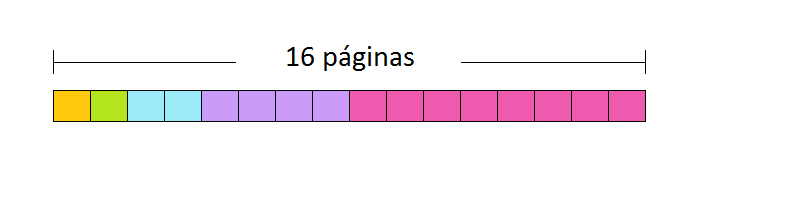
\includegraphics[scale=0.6]{imagem4.png}
\end{figure}

\begin{itemize}

\item Verifica se o tamanho é menor ou igual a sua metade

\item Caso o tamanho do processo não seja dos listados acima, o First Fit é acionado

\item Remoção: checa o intervalo do espaço livre para atualização das listas

\end{itemize}

\justifying
\end{frame}



%------------------------------------------------
\section{Substituição de Página}
%------------------------------------------------
\begin{frame}
\begin{LARGE}
\begin{center}
Substituição de Página
\end{center}
\end{LARGE}
\end{frame}

%------------------------------------------------
\begin{frame}
\frametitle{MMU}
\begin{itemize}

\item Base dos processos obtidos a partir de um dicionário: 

[ pid ][ base ][ limite ]

\item Mapa MMU: 
 
[ bit presente / ausente ][ page frame ][ bit R ][ contador ]

\item (Base + endereço local) do processo --- mapeamento --- endereço físico

\end{itemize}
\justifying
\end{frame}

%------------------------------------------------
\begin{frame}
\frametitle{MMU}
Como funciona?
\begin{enumerate}

\item Verifica local da sua base (Dicionário)

\item Verifica se página solicitada (base + local) possui bit presente = 1

\item Se sim: mapeia para o endereço físico

\item Se não:  checa se a memória física possui espaço para a página (First Fit)

\item Se sim: copia a página para memória física

\item Se não: Substituição de página

\end{enumerate}
\justifying
\end{frame}


%------------------------------------------------
%\begin{frame}
%\frametitle{MMU}
%IMAGEM MAPEAMENTO MMU
%\justifying
%\end{frame}


%------------------------------------------------
\begin{frame}
\frametitle{MMU}
\begin{itemize}
\item Função que reseta o bit R do mapa a cada k segundos [Lock prioritário]

\item Bit M desconsiderado
\end{itemize}

\justifying
\end{frame}


%------------------------------------------------
\subsection{NRUP} 
%------------------------------------------------
\begin{frame}
\frametitle{Not Recently Used Page}

\begin{center}
[ pid ][ frame ][ bit R ][ contador ]
\end{center}

\begin{itemize}

\item Dentre as páginas presentes na memória física, checa qual deles possui R = 0

\item Caso todos os bits R’s = 1, espera resetar os bits R’s
\end{itemize}
\justifying
\end{frame}

%------------------------------------------------
\subsection{FIFO} 
%------------------------------------------------
\begin{frame}
\frametitle{First-In First-Out}

\begin{center}
[ pid ][ frame ][ bit R ][ contador ]
\end{center}

\begin{itemize}
\item Coloca na fila as páginas dos processos que foram ocupando a memória física

\item A página mais ‘velha’ é retirada
\end{itemize}
\justifying

\end{frame}

%------------------------------------------------
\subsection{Second Chance} 
%------------------------------------------------
\begin{frame}
\frametitle{Second Chance}

\begin{center}
[ pid ][ frame ][ bit R ][ contador ]
\end{center}

\begin{itemize}
\item Coloca na fila as páginas dos processos que foram ocupando a memória física

\item Verifica se a página a ser retirada possui bit R = 0

se sim: a página é retirada

se não: bit R é resetado e o processo é colocado no final da fila.
\end{itemize}
\justifying
\end{frame}

%------------------------------------------------
\begin{frame}
\frametitle{Second Chance}
Obs:
\begin{itemize}
\item Os bits R’s das páginas que estão na fila podem ser resetados

\item Caso uma página tenha bit R = 0 e seja referenciada por algum processo, esse bit R permanecerá com bit R = 0
\end{itemize}
\justifying
\end{frame}


%------------------------------------------------
\subsection{LRUP}
%------------------------------------------------
\begin{frame}
\frametitle{Least Recently Used Page}

\begin{center}
[ pid ][ frame ][ bit R ][ contador ]
\end{center}

\begin{itemize}
\item Utiliza o contador e o bit R como referência

\item A cada pulso de "clock" soma ao contador o valor de R
\end{itemize}
\justifying
\end{frame}

%------------------------------------------------
\section{Resultados} 
%------------------------------------------------
\begin{frame}
\begin{LARGE}
\begin{center}
Resultados
\end{center}
\end{LARGE}
\end{frame}

%------------------------------------------------
\begin{frame}
\frametitle{Gerenciamento de Espaço Livre} 

\justifying
\end{frame}


%------------------------------------------------
\begin{frame}
\frametitle{Substituição de Páginas} 
\justifying
\end{frame}


\end{document}
